\chapter{Principal Component Analysis}
\label{chapter:pca}
\section{簡介}
\label{sec:background}


在機器學習中,資料的特徵(維度)數往往會影響模型的訓練效果,特徵太少可能所包含的資訊量太少,在進行模型訓練時,往往無法順利將資料進行正確的分類,所以會僅可能收集與資料集相關的特徵。但當資料的特徵多到一定的程度時,卻會因爲所包含的資訊太多,導致訓練出來的模型過擬合的現象,以至於分類器的效果不增反減,這種現象我們稱爲「維度災難」,如圖\ref{fig:curse_of_dimesionality}所示。所以在資料特徵過多的情況下,會進行資料降維,將一些特徵刪除,盡可能的減少模型發生過擬的現象,進而增加模型的訓練效果。

Principal Component Analysis,是一種非監督式的資料降維演算法,它的運作原理方式是希望在特徵空間中,找出一個投影向量,使得這資料的投影點能有最大的變異量。並分析各個特徵對於變異量共獻,進而刪除共獻量較少的特徵。



\begin{figure}[h]
	\centering
	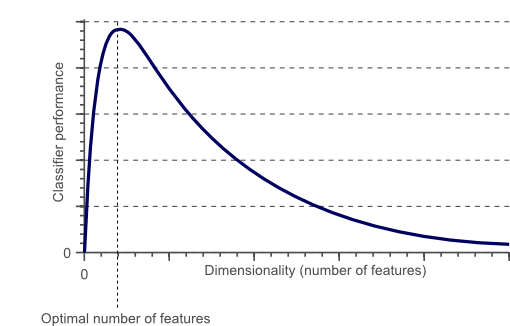
\includegraphics[height=5cm]{./pic/NZgacRXF.png}
	\caption{維度災難示意圖}
	\label{fig:curse_of_dimesionality}
\end{figure}


\subsection{子章節二}
為了更簡單理解這個演算法的數學義意,以下舉一個例子說明:

○○○如圖~\ref{fig:types_comparison}所示。
\begin{figure}[!t]
	\begin{center}
		\begin{tabular}{ccccccccccccc}
			\subfigure[類型A]{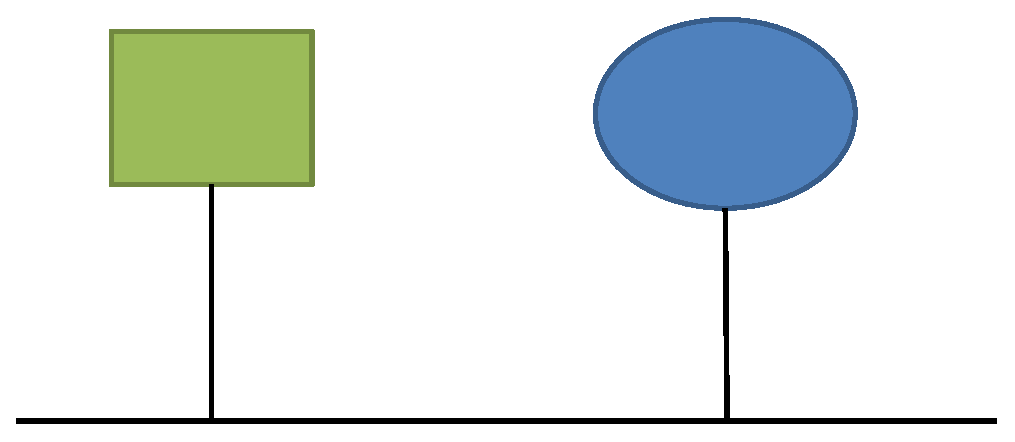
\includegraphics[height=2.4cm]{graphs/introduction/typeA.eps}\label{fig:typeA} } \par &
			\subfigure[類型B]{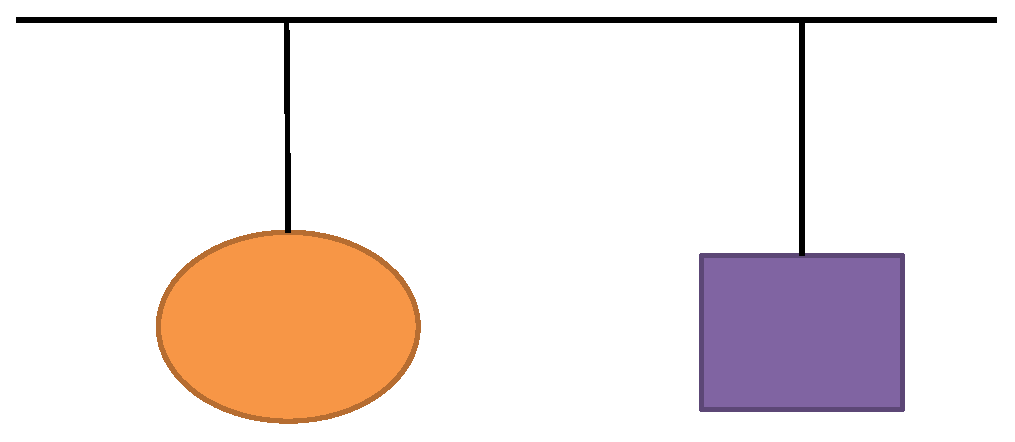
\includegraphics[height=2.4cm]{graphs/introduction/typeB.eps}\label{fig:typeA} } \par   \\
		\end{tabular}
		\caption{○○○比較}
		\label{fig:types_comparison}
	\end{center}
\end{figure}

\section{○○○問題與處理機制}
問題與機制,問題與機制,問題與機制,問題與機制,
問題與機制,問題與機制,問題與機制,問題與機制,
問題與機制,問題與機制,問題與機制,問題與機制,
問題與機制,問題與機制,問題與機制,問題與機制,
問題與機制。

%要被單行註解的文字。

\begin{comment}
要被區塊註解的文字,要被區塊註解的文字,要被區塊註解的文字,
要被區塊註解的文字,要被區塊註解的文字,要被區塊註解的文字,
要被區塊註解的文字,要被區塊註解的文字,要被區塊註解的文字,
要被區塊註解的文字,要被區塊註解的文字,要被區塊註解的文字,
要被區塊註解的文字,要被區塊註解的文字,要被區塊註解的文字,
要被區塊註解的文字,要被區塊註解的文字。
\end{comment}

\section{研究動機與目的}
動機與目的,動機與目的,動機與目的,動機與目的,
動機與目的,動機與目的,動機與目的,動機與目的,
動機與目的,動機與目的,動機與目的,動機與目的,
動機與目的,動機與目的,動機與目的,動機與目的,
動機與目的,動機與目的,動機與目的,
細節如表\ref{tab:mytitle1}。
\begin{table}[!t]
	\centering
	\caption{表格標題1}
	\label{tab:mytitle1}
	% Table generated by Excel2LaTeX from sheet 'table_01'
\begin{tabular}{rr}
\toprule
Title & Values \\
\midrule
A     & 1612 \\
B     & 256 \\
C     & 30 \\
D     & 7 \\
E     & 3 \\
\bottomrule
\end{tabular}%

\end{table}

\begin{enumerate}
	\item
	      列舉一。
	      %
	\item
	      列舉二。
	      %
	\item
	      列舉三。
	      %
\end{enumerate}

\section {研究方法與論文架構}
研究方法與論文架構,研究方法與論文架構,研究方法與論文架構,
研究方法與論文架構,研究方法與論文架構,研究方法與論文架構,
研究方法與論文架構,研究方法與論文架構,研究方法與論文架構,
研究方法與論文架構。

\begin{itemize}
	\item
	      項目一。
	      %
	\item
	      項目二。
	      %
	\item
	      項目三。
	      %
	\item
	      項目四。
\end{itemize}

流程圖如\ref{fig:ResearchFlowChart}。
\begin{figure}[htbp]
	\centering
	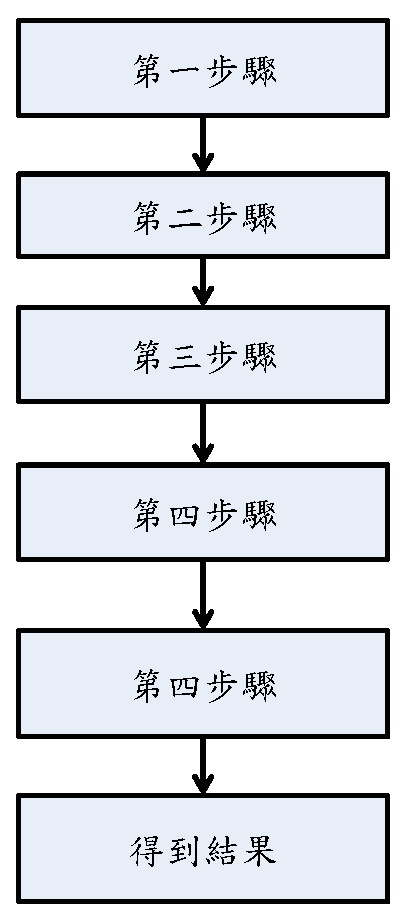
\includegraphics[height=8cm]{graphs/introduction/ResearchFlowChart.eps}
	\caption{研究進行流程圖}
	\label{fig:ResearchFlowChart}
\end{figure}
3
